When the server starts it will execute a method called \code{listen()} that listens for any connections, see \listref{code:listen}.
Whenever any \code{Socket} connects to the server, the \code{listen()} method will create a new \code{CommunicationThread}.
This thread will then read the information in the \code{Socket}'s \code{InputStream} and depending on the connection type (commit event, request event or ping) it will deal with it appropriately.

\lstinputlisting[label=code:listen,caption=Method: \code{listen()}]{code/IOHandler-listen.txt}

In the following subsections we will explain how the different types of connections are processed by the system.


\subsubsection{Ping}
\label{sec:IOPing}

Diagram ledger: (see \figref{fig:IOLedger})\newline
The uppermost port is used to indicate input and the lowermost port is used to indicate output. The arrows indicate which way the information is forwarded in the system. Any arrows leading to and fro a component, and not from an input or output port, are to be executed first.	\newline
\begin{figure}[H]
	\centering
		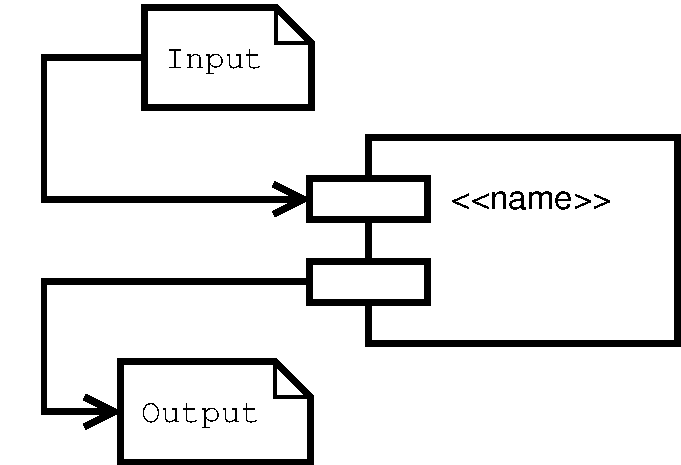
\includegraphics[scale=0.40]{images/ledger.pdf} %FIXME epstopdf package fucker, har ændret noget her
	\caption{Ledger for diagrams}
	\label{fig:IOLedger}
\end{figure}

%	The \newlines are to prevent the words from "running" out of the page - don't know why this happens :(
% This has been tested with   \texttt{arg} and \code{arg}
Figure \ref{fig:IOPing} is a model of how a ping is process by the server. The \code{Connection} component sends output, in this case a ping event, to the server. In the server this is received by the \code{IOHandler}, which creates a new \newline \code{CommunicationThread}.
The \code{CommunicationThread} will then use the \newline \code{TransmissionHandler} to determine if the input is of the type commit, request or ping.
In this case the input is of the type ping, and it will just directly respond to the caller (connection).
\begin{figure}[htbp]
	\centering
          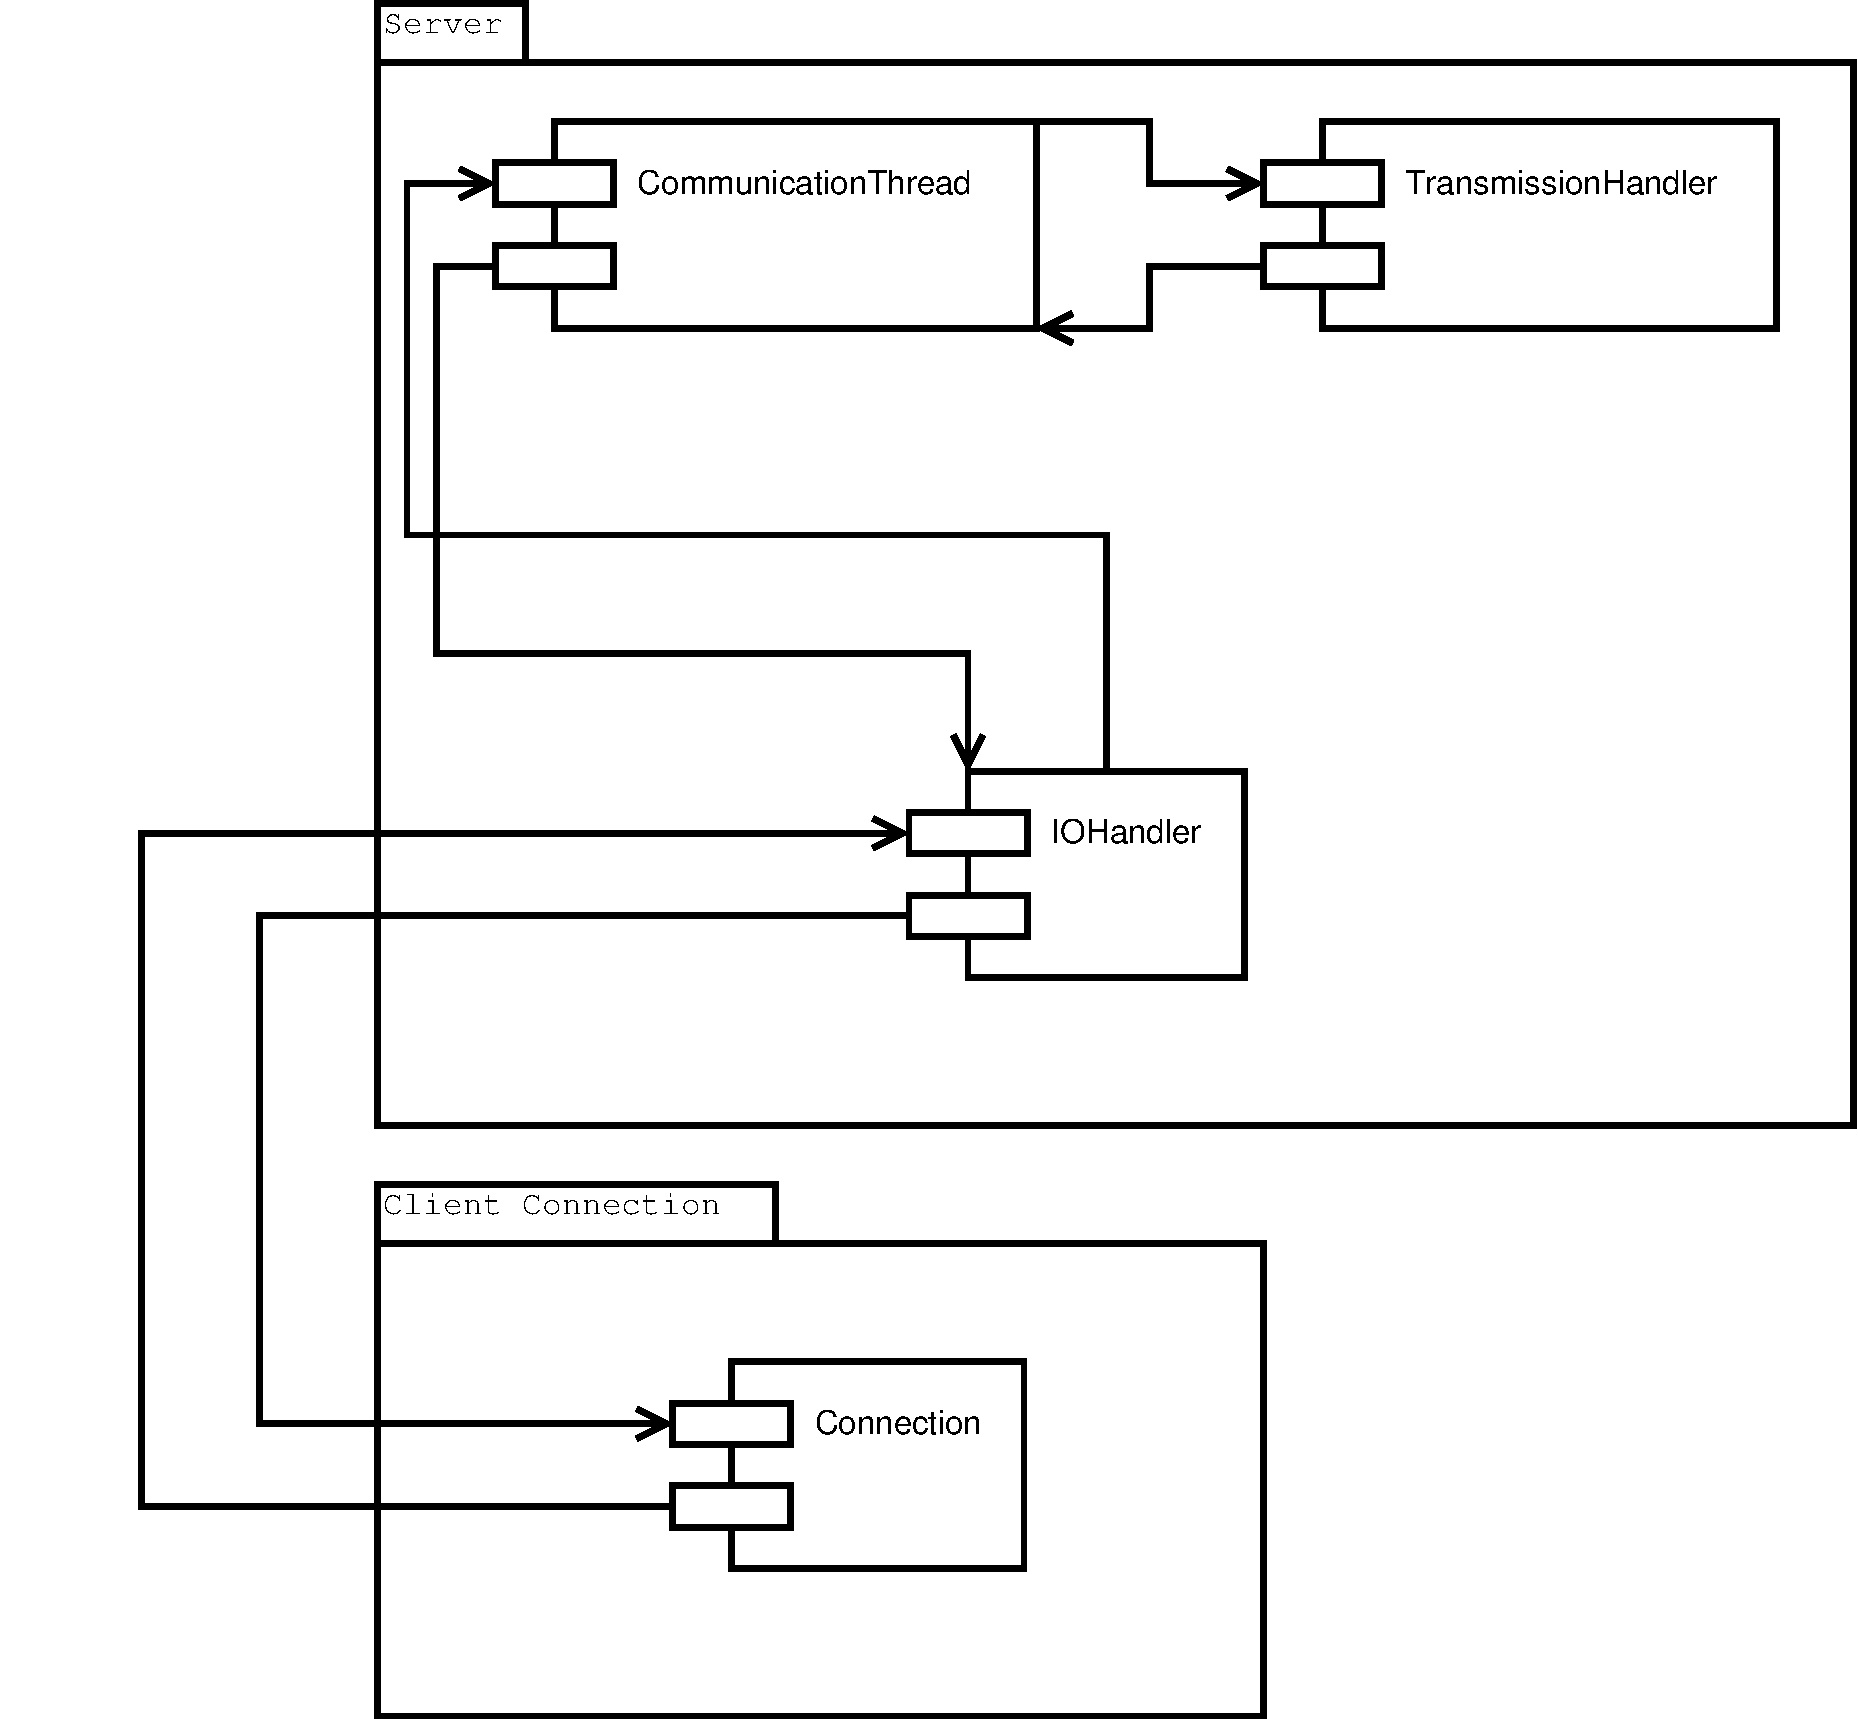
\includegraphics[scale=0.30]{images/ping.pdf}%FIXME epstopdf packager fucker, har ændret til at bruge de generede pdf filer direkte
	\caption{A diagram illustrating how a ping is processed.} 
	\label{fig:IOPing}
\end{figure}

%	The \newlines are to prevent the words from "running" out of the page - don't know why this happens :(
% This has been tested with   \texttt{arg} and \code{arg}
The reason for this implementation is that Java only supports two types of sockets: stream based (TCP --- \code{java.net.Socket} and \code{java.net.ServerSocket}) and datagram based ones (UDP --- \code{java.net.DatagramSocket} \newline and \code{java.net.MulticastSocket})\cite{ICMP}\cite{javaNET}. However an implementation of ping would require the use of ICMP(Internet Control Message Protocol) ping, and since this is not possible we have chose to implement a ping at a software level, rather than as a protocol.


\subsubsection{Commit and Request}
\label{sec:IOCR}
For a connection of type commit or request, the procedure is almost the same. However, when the \code{CommunicationThread} has been created and its \code{TransmissionHandler} has determine the type of the connection, it will opposite for the ping, create a new event corresponding to the type and send it to the \code{EventHandler}, see \figref{fig:IOCR}.
First when the \code{EventHandler} is done processing the event, will the server respond to the connector.
To see how the \code{EventHandler} processes the given queries see \secref{QQHandling}.

\begin{figure}[htbp]
	\centering
		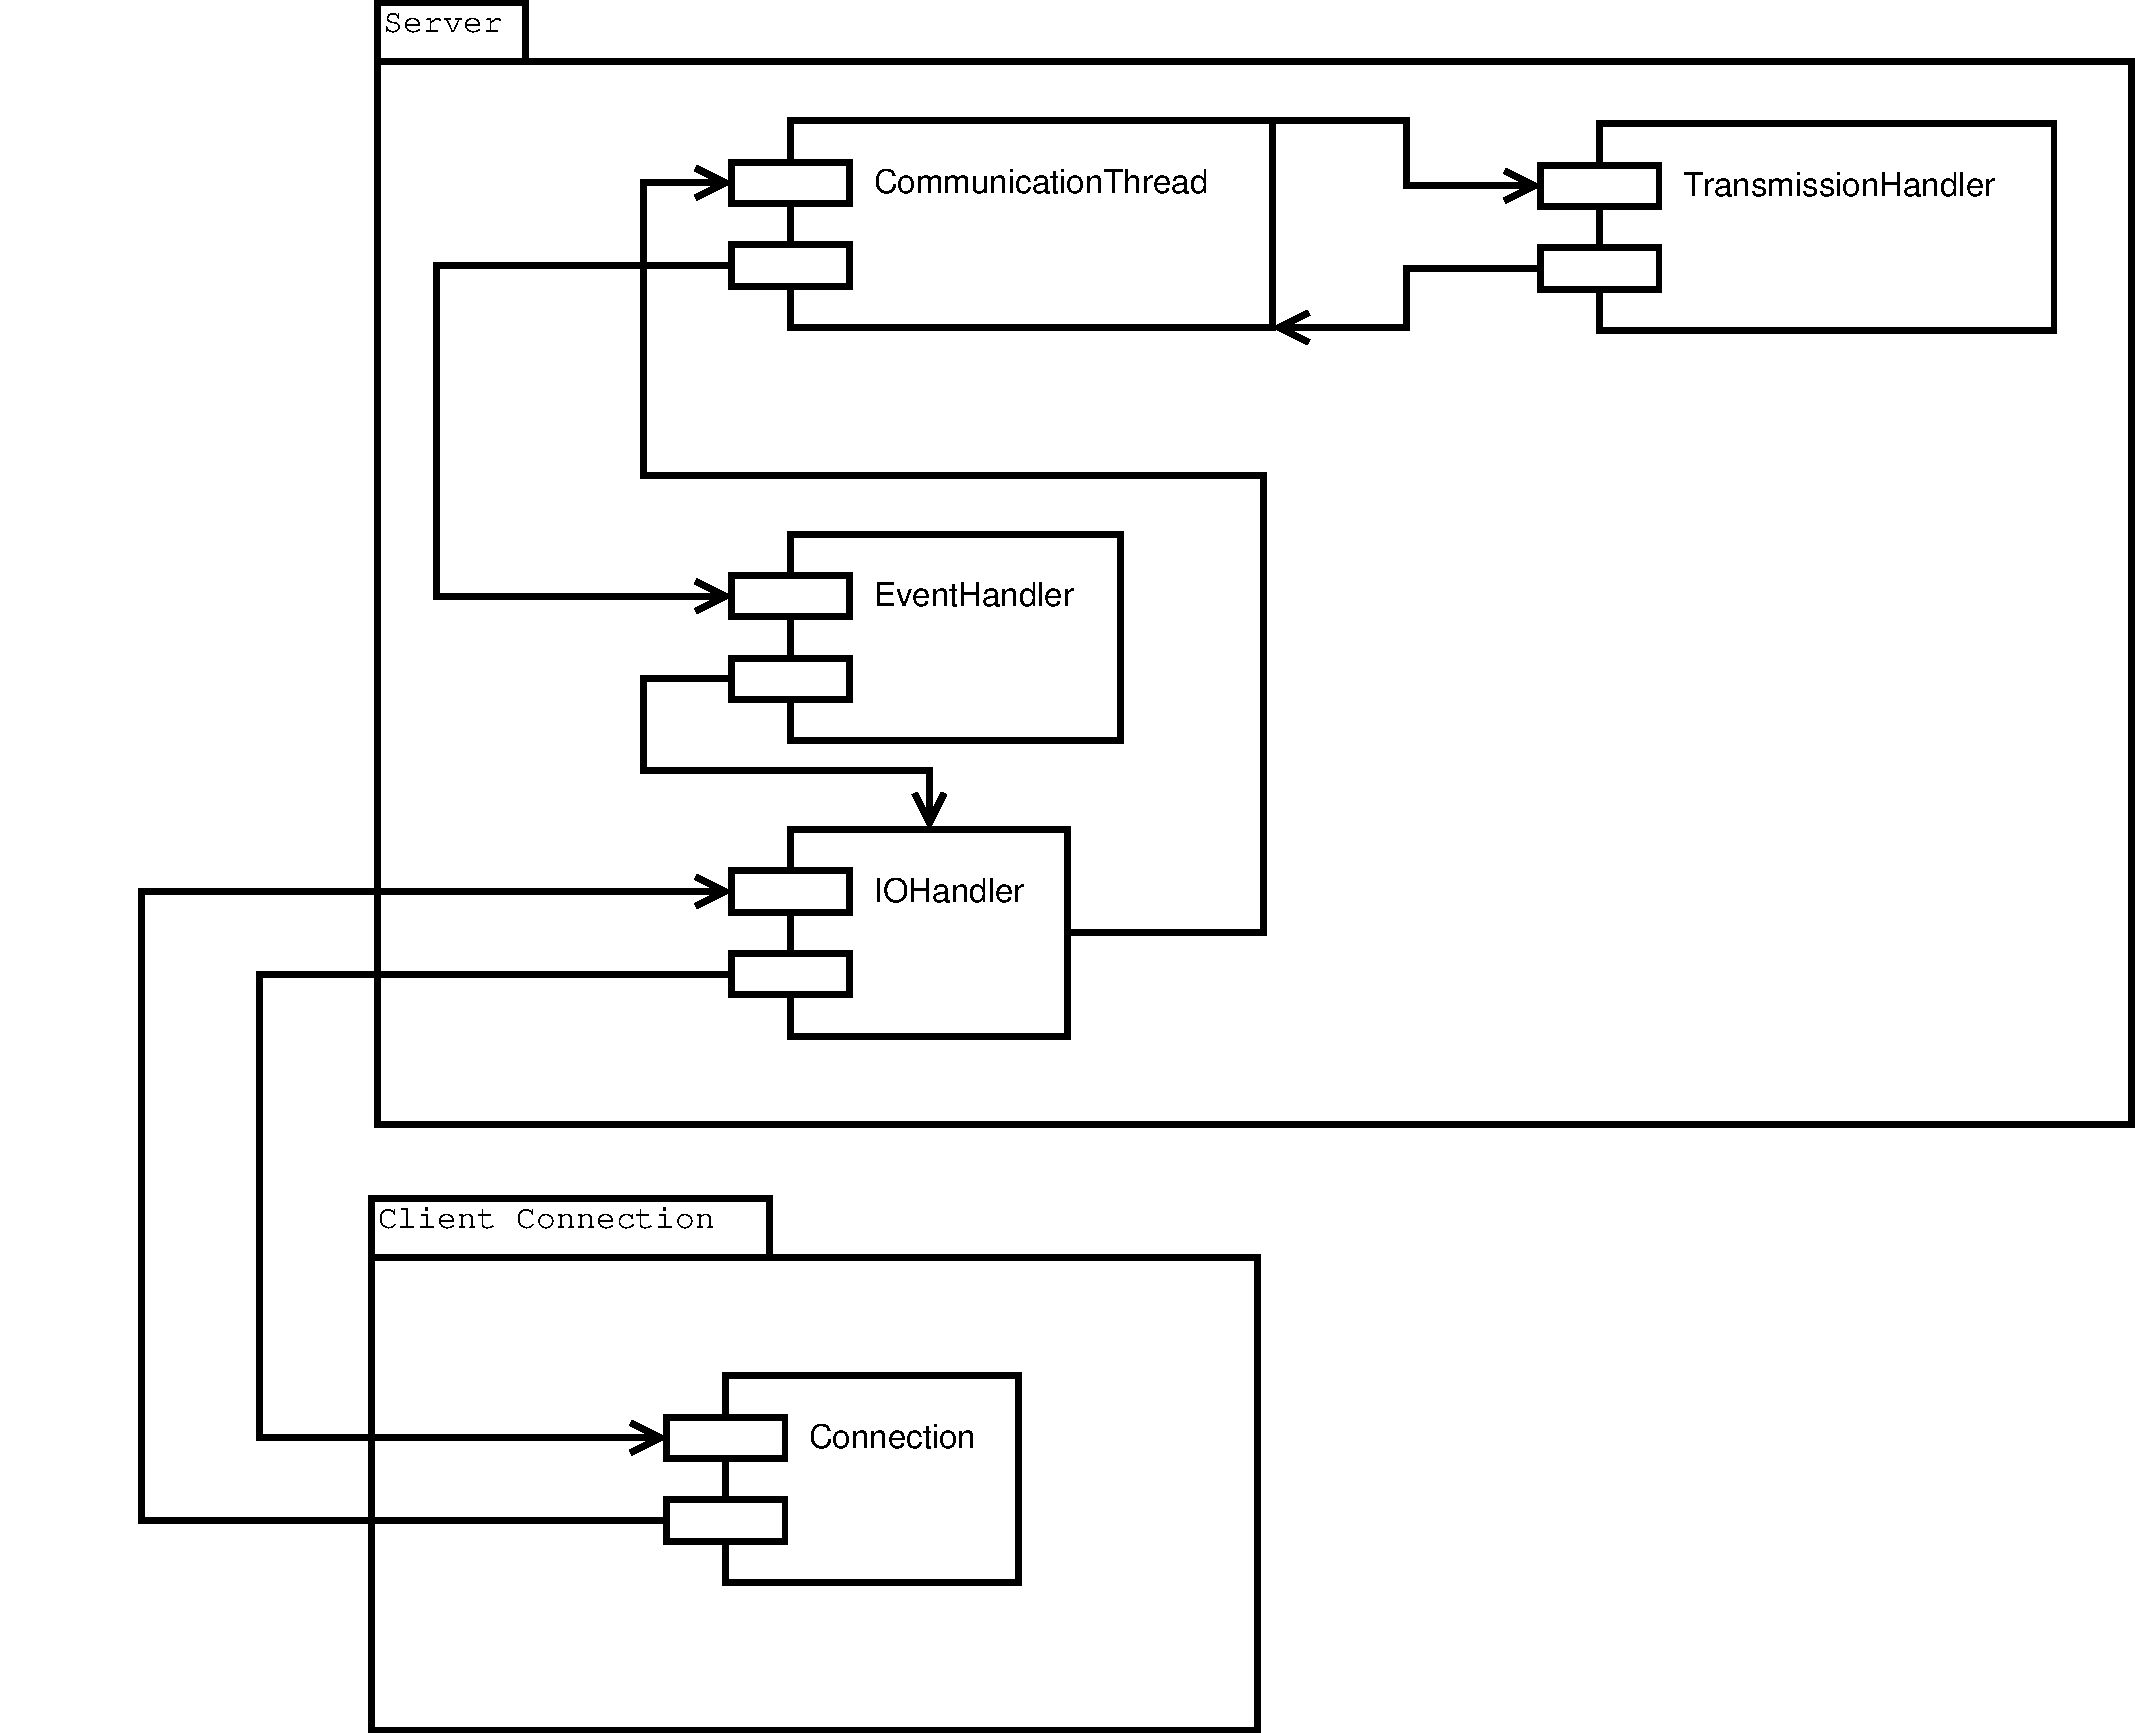
\includegraphics[scale=0.30]{images/requestCommit}
	\caption{A diagram illustrating how a request or a commit event is processed.}
	\label{fig:IOCR}
\end{figure}